\documentclass[border=10pt,varwidth]{standalone}
\usepackage{tikz}
\usetikzlibrary{shapes,arrows,shapes.multipart, positioning}

\begin{document}

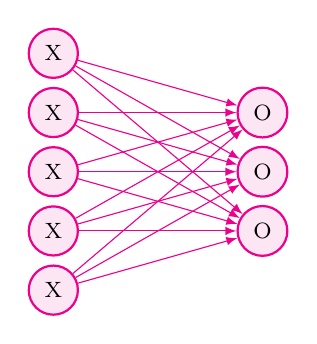
\begin{tikzpicture}
    \tikzset{
        component/.style = {rectangle, draw=magenta,  fill=magenta!10, thick, rounded corners},
        neurone/.style = {circle, draw=magenta, fill=magenta!10, thick, radius=10},
        line/.style = {draw=magenta, thin, -latex}
    }

    \node[neurone](i_1){\footnotesize{X}};
    \node[neurone](i_2)[below = 0.1cm of i_1]{\footnotesize{X}};
    \node[neurone](i_3)[below = 0.1cm of i_2]{\footnotesize{X}};
    \node[neurone](i_4)[below = 0.1cm of i_3]{\footnotesize{X}};
    \node[neurone](i_5)[below = 0.1cm of i_4]{\footnotesize{X}};


    \node[neurone](o_1)[right = 2cm of i_2]{\footnotesize{O}};
    \node[neurone](o_2)[right = 2cm of i_3]{\footnotesize{O}};
    \node[neurone](o_3)[right = 2cm of i_4]{\footnotesize{O}};

    \path [line] (i_1) -- (o_1);
    \path [line] (i_1) -- (o_2);
    \path [line] (i_1) -- (o_3);

    \path [line] (i_2) -- (o_1);
    \path [line] (i_2) -- (o_2);
    \path [line] (i_2) -- (o_3);

    \path [line] (i_3) -- (o_1);
    \path [line] (i_3) -- (o_2);
    \path [line] (i_3) -- (o_3);

    \path [line] (i_4) -- (o_1);
    \path [line] (i_4) -- (o_2);
    \path [line] (i_4) -- (o_3);

    \path [line] (i_5) -- (o_1);
    \path [line] (i_5) -- (o_2);
    \path [line] (i_5) -- (o_3);
    
\end{tikzpicture}

\end{document}
